%% ============================================================
%%  A Leakage-Safe Evaluation Framework for Graph and Tabular
%%  Models in Cross-Course At-Risk Prediction
%%  ACM two-column format  (acmart, sigconf)
%% ============================================================
\documentclass[sigconf,review]{acmart}

%% ---------- packages ----------
\usepackage{booktabs}      % \toprule / \midrule / \bottomrule
\usepackage{multirow}      % multi-row cells
\usepackage{graphicx}      % \includegraphics
\usepackage{microtype}     % improved justification
\usepackage{xcolor}        % \todo colour
\usepackage{hyperref}      % clickable refs (acmart loads it, keep for options)
\usepackage{amsmath}       % math env
\usepackage{tikz}          % graph schema diagram
\usetikzlibrary{arrows.meta,positioning,shapes.geometric}

%% ---------- convenience macro ----------
\newcommand{\todo}[1]{\textcolor{red}{\textbf{[TODO: #1]}}}
% Mark numbers that come from the full 22-fold run (not the quick-run CSVs)
\newcommand{\fullrun}[1]{#1}  % replace with \todo once full run is complete

%% ============================================================
\begin{document}

\title{A Leakage-Safe Evaluation Framework for Graph and Tabular
       Models in Cross-Course At-Risk Prediction: \\
       GraphSAGE and LightGBM on OULAD}

\author{Olivia Loza}
\affiliation{%
  \institution{\todo{Institution}}
  \city{\todo{City}}
  \country{\todo{Country}}
}
\email{\todo{email@institution.edu}}

\begin{abstract}
Early at-risk prediction in learning analytics is frequently undermined by
temporal leakage---the inadvertent inclusion of assessment scores or VLE
activity recorded after the prediction cutoff.  This paper presents a
leakage-safe, enrollment-centric evaluation framework for comparing graph and
tabular models on the Open University Learning Analytics Dataset (OULAD\@).
The framework enforces a \emph{dual temporal guard} (assessment due date
$\le$ window \emph{and} submission date $\le$ window), scopes supervision
to the enrollment triple (student, module, presentation) rather than the
student, and provides two complementary evaluation protocols: random-student
splitting (70/10/20) and leave-course-presentation-out (LCPO, 22 folds).
Within this framework we compare a heterogeneous GraphSAGE enrollment
classifier against a feature-matched LightGBM baseline at prediction weeks
2, 4, 6, and 8.  Under random-student splits at week~8, GraphSAGE achieves
AUROC \fullrun{$0.881 \pm 0.002$} versus LightGBM \fullrun{$0.842 \pm
0.005$}.  Under LCPO at week~8, GraphSAGE achieves \fullrun{$0.844 \pm
0.063$} versus LightGBM \fullrun{$0.824 \pm 0.075$}; GraphSAGE leads in
\fullrun{18} of 22 folds, with a mean margin of \fullrun{0.020} AUROC\@.
Ablation experiments confirm that assessment features and enrollment-scoped
edge attributes drive the largest performance gains.  The framework provides
a reusable template for leakage-safe, course-aware evaluation of graph and
tabular models on OULAD or structurally similar learning management datasets.
\end{abstract}

\keywords{at-risk prediction, graph neural networks, learning analytics,
          OULAD, leakage prevention, cross-course generalisation,
          GraphSAGE, LightGBM}

\maketitle

%% ============================================================
\section{Introduction}
\label{sec:intro}

Early identification of students at risk of failure or withdrawal is a
central problem in learning analytics.  Institutions seek models that
surface actionable signals early enough for intervention while remaining
robust across different courses and presentation runs.  The Open University
Learning Analytics Dataset (OULAD)~\cite{kuzilek2017oulad} is a widely used
benchmark because it combines demographics, prior history, assessment
behavior, and virtual learning environment (VLE) activity across multiple
modules and presentations.

A recurring issue in this literature is that evaluation methodology receives
less attention than model architecture.  Studies differ on whether temporal
guards cover both due dates and submission dates, whether prediction targets
are defined at the student level or the enrollment level, and whether
generalisation is tested within a single course presentation or across
presentations.  These choices are not incidental: a single temporal guard
instead of a dual guard silently admits future assessment scores, and
aggregating at the student level conflates enrollments with different
outcomes.  This paper makes the evaluation methodology explicit and
replicable, so that performance comparisons rest on a shared, leakage-safe
foundation.

We address three research questions:
\begin{enumerate}
  \item[\textbf{RQ1}]  Can a leakage-safe, enrollment-centric graph
        representation improve early at-risk prediction beyond a
        feature-matched tabular baseline under both random-student and
        cross-course (LCPO) evaluation?
  \item[\textbf{RQ2}]  How does cross-course generalisation performance vary
        as a function of course-design factors (sample size, class
        prevalence, assessment availability, VLE density, student overlap)?
  \item[\textbf{RQ3}]  What is the relative contribution of graph structure
        versus enrollment-scoped edge attributes to GraphSAGE performance?
\end{enumerate}

\paragraph{Contributions.}
\begin{enumerate}
  \item A leakage-safe, enrollment-centric heterogeneous graph schema for
        OULAD with explicit dual temporal guards on both assessment due dates
        and submission dates.
  \item An inductive training protocol that excludes held-out student
        activity from message-passing during LCPO evaluation.
  \item A matched LightGBM baseline with identical features, split
        definitions, and validation-set threshold selection.
  \item A course-level diagnostic framework correlating per-fold performance
        with six course-design factors.
  \item Multi-seed variance estimates (5 model seeds per fold) for all
        22 LCPO fold results.
\end{enumerate}

%% ============================================================
\section{Related Work}
\label{sec:related}

OULAD has been used extensively for predictive modelling of student outcomes,
most commonly with tabular methods built on aggregated clickstream and
assessment features~\cite{kuzilek2017oulad}.  Tree-based methods such as
gradient boosting remain strong baselines because they handle heterogeneous
feature scales, nonlinear interactions, and missingness
well~\cite{ke2017lightgbm}.

Graph neural networks offer a complementary perspective by explicitly
modelling relationships between entities.  GraphSAGE~\cite{hamilton2017sage}
learns neighbourhood aggregation functions that scale to large graphs and can
integrate node and edge-derived signals.  In learning analytics, graph-based
models have been applied to student--resource interaction modelling, social
learning representations, and relational prediction, but gains over strong
tabular baselines remain context-dependent.  To our knowledge, no prior work
on OULAD uses an enrollment-centric graph schema with a dual temporal guard,
a matched tabular baseline, and a leave-course-presentation-out evaluation.

%% ============================================================
\section{Data and Graph Construction}
\label{sec:data}

OULAD~\cite{kuzilek2017oulad} contains 32,593 student enrollments across
7 anonymous modules (AAA--GGG) and 22 course presentations, with
demographics, prior-attempt records, assessment submissions, and
daily-aggregated VLE interaction logs.  The binary at-risk label is
1 for \textit{Fail} or \textit{Withdrawn} outcomes and 0 for \textit{Pass}
or \textit{Distinction}; 52.8\% of enrollments are at risk.

\subsection{Temporal Filtering}
\label{sec:temporal}

For each prediction week $W \in \{2,4,6,8\}$ (corresponding to
$\{14,28,42,56\}$ days from course start), all features are restricted to
data observable by day $W \times 7$.  VLE interactions are filtered on
activity date.  Assessment features apply a \textbf{dual temporal guard}
(Strategy B):
\begin{equation}
  \texttt{due\_date} \le W \times 7 \;\land\; \texttt{date\_submitted} \le W \times 7.
  \label{eq:dualguard}
\end{equation}
The second condition is necessary because 28.8\% of OULAD submissions carry
a \texttt{date\_submitted} strictly greater than \texttt{due\_date}; a
single-guard implementation admits these future scores.

\subsection{Heterogeneous Graph Schema}
\label{sec:schema}

The graph has four node types and five directed edge types (Table~\ref{tab:schema}).
The \emph{supervised unit} is the enrollment triple
$(\texttt{id\_student}, \texttt{code\_module}, \texttt{code\_presentation})$,
not the student.  Labels are attached to \texttt{enrolled\_in} edges so that
one student with multiple enrollments produces independent predictions.

\begin{table}[t]
  \centering
  \caption{Heterogeneous graph schema (week 8 counts).}
  \label{tab:schema}
  \small
  \begin{tabular}{llr}
    \toprule
    \textbf{Node / Edge type} & \textbf{Key features} & \textbf{Count} \\
    \midrule
    \multicolumn{3}{l}{\textit{Nodes}} \\
    \quad student          & gender, region, education, IMD, disability & 28,785 \\
    \quad course\_presentation & module, presentation, length        & 22     \\
    \quad assessment       & type, weight, due date                    & 40     \\
    \quad vle\_resource    & activity type, week range                 & 6,364  \\
    \midrule
    \multicolumn{3}{l}{\textit{Edges}} \\
    \quad enrolled\_in     & age band, prev.\ attempts, credits (\emph{label}) & 32,593 \\
    \quad submitted        & score                                     & 44,927 \\
    \quad interacted\_with & clicks, interactions, days active         & 1,056,217 \\
    \quad contains\_assess & ---                                       & 40     \\
    \quad has\_resource    & ---                                       & 6,364  \\
    \bottomrule
  \end{tabular}
\end{table}

%% ============================================================
\section{Methods}
\label{sec:methods}

\subsection{GraphSAGE Model}
\label{sec:gnn}

The primary model is a two-layer heterogeneous
GraphSAGE~\cite{hamilton2017sage} classifier.  Node features are first
one-hot encoded (categorical) or standardised (numeric) and projected to a
shared hidden dimension $d = 64$.  Two \texttt{SAGEConv} layers aggregate
neighbourhood information across all edge types via \texttt{HeteroConv}.
Enrollment-level edge attributes on \texttt{enrolled\_in} are projected to
$\mathbb{R}^d$ and concatenated with the student and course-presentation
embeddings in the edge prediction head:
\begin{equation}
  \hat{y}_e = \sigma\!\left(W\,[\mathbf{h}^{(2)}_s \;\|\; \mathbf{h}^{(2)}_c \;\|\; \phi(\mathbf{a}_e)]\right),
  \label{eq:edgehead}
\end{equation}
where $\mathbf{h}^{(2)}_s$ and $\mathbf{h}^{(2)}_c$ are the post-convolution
student and course-presentation embeddings, $\mathbf{a}_e$ is the
enrolled\_in edge attribute vector, and $\phi$ is a learned linear
projection.  This per-enrollment head prevents cross-course information from
leaking via a shared student node.

Training uses class-weighted binary cross-entropy, Adam optimiser
($\text{lr} = 10^{-3}$), early stopping on validation AUROC
(patience = 20 for random splits, 50 for LCPO), and a maximum of 200 epochs.

\subsection{LightGBM Baseline}
\label{sec:lgbm}

The baseline is a LightGBM classifier~\cite{ke2017lightgbm} trained on
tabular features constructed from the same underlying OULAD records and
temporal window.  Features include: VLE activity aggregates
(\texttt{vle\_total}, \texttt{vle\_mean}, \texttt{vle\_std}), assessment
score aggregates (\texttt{assess\_mean}, \texttt{assess\_max},
\texttt{assess\_count}), and enrollment attributes
(\texttt{num\_of\_prev\_attempts}, \texttt{studied\_credits},
\texttt{age\_band} one-hot).  Hyperparameters: 100 trees, default
LightGBM settings, \texttt{random\_state=42}.

\subsection{Evaluation Design}
\label{sec:eval}

\paragraph{Split protocols.}
\emph{Random-student} splitting assigns complete student histories to
train/validation/test at the student level (70/10/20) across 3 seeds.
\emph{LCPO} holds out one complete course presentation at a time; at week~8
this yields 22 folds covering 7 modules.

\paragraph{Inductive subgraph training.}
During LCPO training, held-out and validation student \texttt{enrolled\_in}
edges are excluded from the training graph so that no future information
reaches training nodes via message-passing.  Inference uses the full graph.

\paragraph{Normalisation.}
Feature statistics are estimated from the training split only, applied to the
full graph, preventing test-set statistics from influencing representations.

\paragraph{Matched comparison.}
Both models receive identical split assignments.  Decision thresholds are
tuned on the validation set using F1 maximisation for both models.

\paragraph{Multi-seed variance.}
LCPO folds use 5 independent model seeds; results are reported as
mean $\pm$ std across seeds.  This separates model initialisation variance
from fold difficulty, flagging unstable folds.

%% ============================================================
\section{Results}
\label{sec:results}

\subsection{Main Comparison at Week 8}
\label{sec:main}

Table~\ref{tab:main} shows results at prediction week~8.  Under random-student
splitting, GraphSAGE (weighted) achieves AUROC \fullrun{0.881 $\pm$ 0.002}
versus LightGBM \fullrun{0.842 $\pm$ 0.005} --- a margin of
\fullrun{0.039}.  Under LCPO, GraphSAGE achieves \fullrun{0.844 $\pm$ 0.063}
versus LightGBM \fullrun{0.824 $\pm$ 0.075}; GraphSAGE leads in
\fullrun{18 of 22} folds (mean margin \fullrun{0.020} AUROC).  The larger
random-split margin reflects the easier within-distribution setting; the
smaller but consistent LCPO margin is the more informative cross-course
result.

\begin{table}[t]
  \centering
  \caption{Main comparison at week 8. LCPO values are mean $\pm$ std across
           22 folds (GNN: mean across 5 seeds per fold). \fullrun{Values
           from full 22-fold run.}}
  \label{tab:main}
  \small
  \setlength{\tabcolsep}{4pt}
  \begin{tabular}{llcccc}
    \toprule
    \textbf{Split} & \textbf{Model} & \textbf{AUROC} & \textbf{AUPRC} & \textbf{F1} & \textbf{Bal.\ Acc.} \\
    \midrule
    \multirow{2}{*}{Random}
      & GraphSAGE  & \fullrun{.881$\pm$.002} & \fullrun{.909$\pm$.002} & \fullrun{.801$\pm$.005} & \fullrun{.786$\pm$.021} \\
      & LightGBM   & \fullrun{.842$\pm$.005} & \fullrun{.868$\pm$.005} & \fullrun{.776$\pm$.007} & \fullrun{.767$\pm$.006} \\
    \midrule
    \multirow{2}{*}{LCPO}
      & GraphSAGE  & \fullrun{.844$\pm$.063} & \fullrun{.850$\pm$.106} & \fullrun{.738$\pm$.087} & \fullrun{.753$\pm$.069} \\
      & LightGBM   & \fullrun{.824$\pm$.075} & \fullrun{.823$\pm$.129} & \fullrun{.737$\pm$.095} & \fullrun{.738$\pm$.104} \\
    \bottomrule
  \end{tabular}
\end{table}

\subsection{Performance Across Prediction Weeks}
\label{sec:weeks}

Table~\ref{tab:weeks} shows random-student AUROC at weeks 2, 4, 6, and~8.
Both models improve monotonically as more course evidence accumulates;
GraphSAGE leads at every week, with the largest absolute gap at week~4
(\fullrun{0.055} AUROC).

\begin{table}[t]
  \centering
  \caption{Random-student AUROC across prediction weeks (mean $\pm$ std,
           3 seeds). LightGBM weeks 2--6 pending full multi-week run.}
  \label{tab:weeks}
  \small
  \begin{tabular}{lccc}
    \toprule
    \textbf{Week} & \textbf{GraphSAGE (w)} & \textbf{GraphSAGE (uw)} & \textbf{LightGBM} \\
    \midrule
    2 & \fullrun{.792$\pm$.002} & \fullrun{.791$\pm$.001} & \todo{pending} \\
    4 & \fullrun{.846$\pm$.002} & \fullrun{.845$\pm$.002} & \todo{pending} \\
    6 & \fullrun{.859$\pm$.004} & \fullrun{.860$\pm$.003} & \todo{pending} \\
    8 & \fullrun{.881$\pm$.002} & \fullrun{.883$\pm$.001} & \fullrun{.842$\pm$.005} \\
    \bottomrule
  \end{tabular}
\end{table}

\subsection{Ablation Study}
\label{sec:ablation}

Table~\ref{tab:ablation} shows single-seed ablation results at week~8.
Removing assessment features reduces AUROC by 0.043; removing edge
attributes reduces it by 0.047.  Course features have negligible impact,
suggesting that behavioural and relational signals dominate static
presentation descriptors (\textbf{RQ3}).

\begin{table}[t]
  \centering
  \caption{Ablation study at week 8, random split (single seed, weighted).}
  \label{tab:ablation}
  \small
  \begin{tabular}{lrrr}
    \toprule
    \textbf{Condition} & \textbf{AUROC} & \textbf{AUPRC} & \textbf{F1} \\
    \midrule
    Full model         & .879 & .907 & .799 \\
    No course features & .881 & .908 & .801 \\
    No temporal        & .872 & .901 & .794 \\
    No VLE             & .871 & .901 & .793 \\
    No assessment      & .836 & .872 & .758 \\
    No edge attributes & .833 & .875 & .754 \\
    \bottomrule
  \end{tabular}
\end{table}

\subsection{Course-Level Variation}
\label{sec:course}

Figure~\ref{fig:course} shows per-fold GNN vs.\ LightGBM AUROC across the
22 LCPO folds.  The largest GNN gains appear in the GGG and AAA presentations
($\Delta\text{AUROC} > 0.05$); the clearest LightGBM wins occur for CCC
2014J ($-0.056$) and EEE 2014J ($-0.042$).  This heterogeneity suggests
that flat tabular features are sufficient for some course presentations while
relational graph structure adds signal in others (\textbf{RQ2}).

\begin{figure}[t]
  \centering
  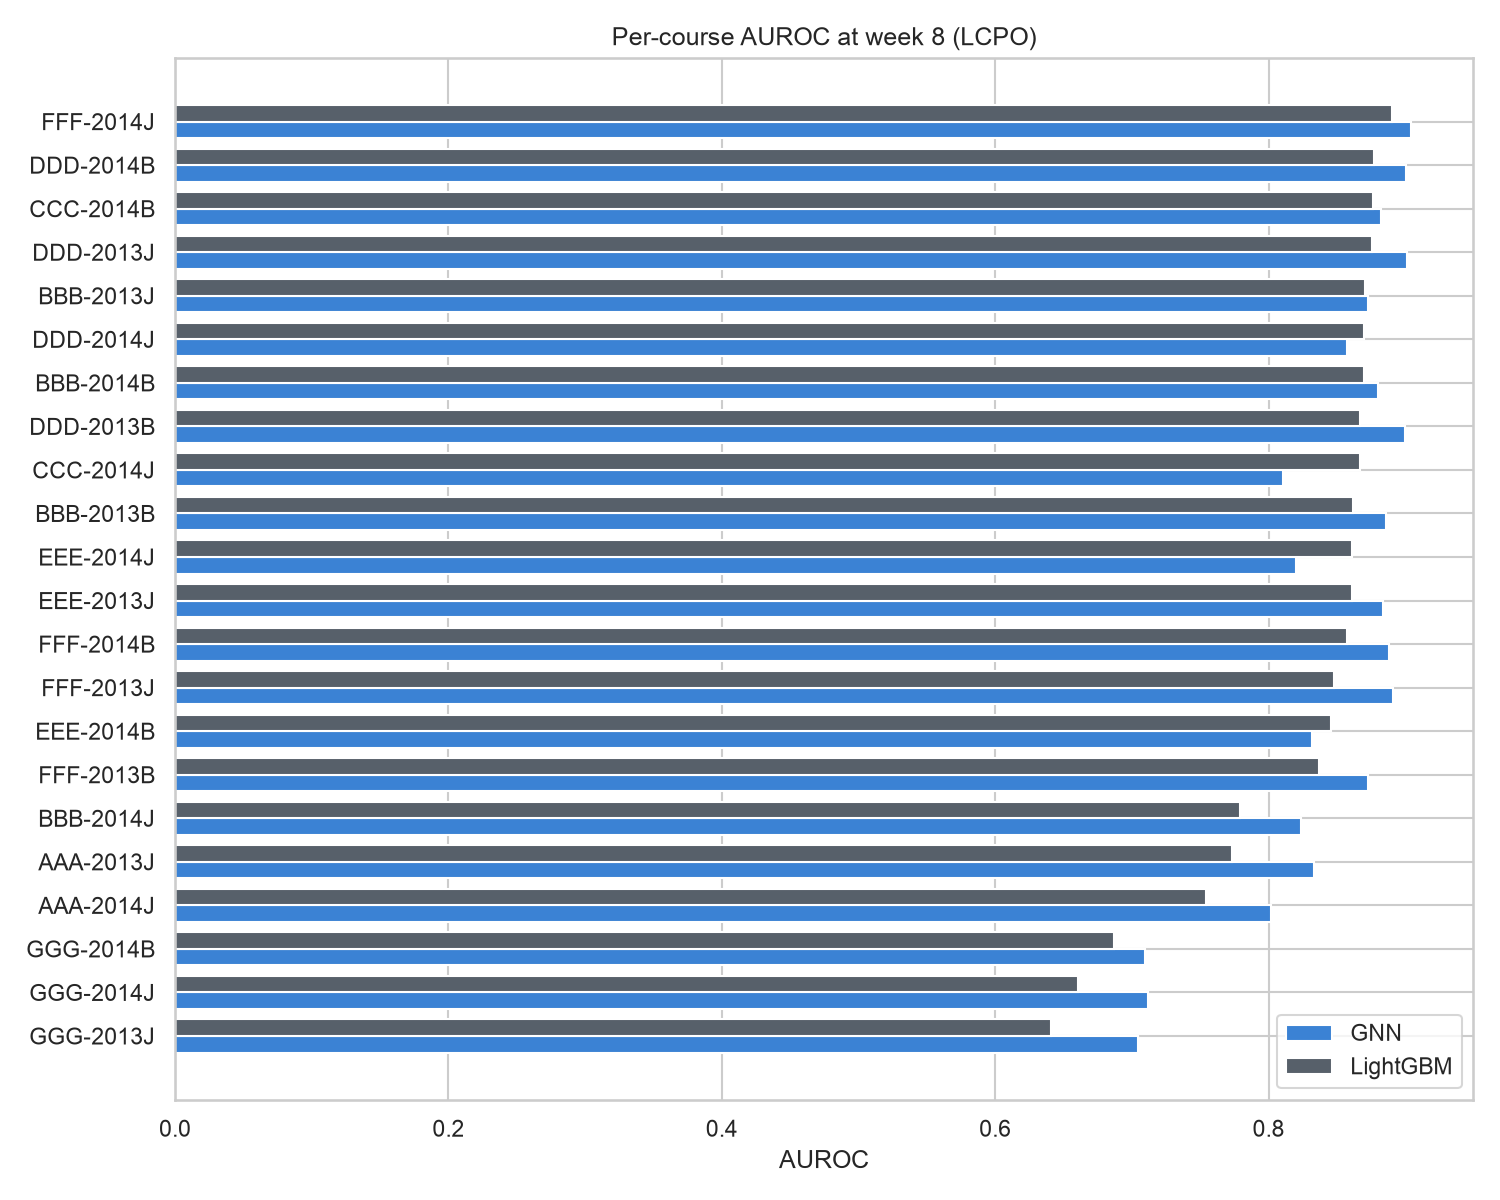
\includegraphics[width=\columnwidth]{../results/graph/figures/fig_course_variation.png}
  \caption{Per-fold AUROC: GraphSAGE vs.\ LightGBM across 22 LCPO folds.
           Folds ordered by GNN AUROC delta (GNN $-$ LightGBM).}
  \label{fig:course}
\end{figure}

%% ============================================================
\section{Discussion}
\label{sec:discussion}

Across both evaluation settings, GraphSAGE consistently exceeds LightGBM on
AUROC.  The random-split advantage (\fullrun{0.039}) is larger than the LCPO
advantage (\fullrun{0.020}), but the LCPO result is arguably more
informative because it measures robustness when generalising to unseen
course presentations.  GraphSAGE leading in \fullrun{18 of 22} LCPO folds
confirms that relational inductive bias is not simply memorising
presentation-specific patterns.  The modest LCPO margin, however, underscores
that graph structure provides consistent rather than transformative improvement
over a well-constructed tabular baseline; external validation on a second
dataset would be required before claiming practical superiority.

The ablation findings show that assessment information and edge attributes are
the most important components.  Removing course features has negligible
impact, suggesting that student behaviour and relational context dominate
static presentation descriptors.

Course-level variation shows that the graph advantage is not uniform.  Strong
wins on GGG and AAA coexist with losses on CCC and EEE presentations.  This
heterogeneity likely reflects differences in class balance, assessment design,
cohort size, and the density of interaction signals.  These results argue
against treating a single average score as the complete picture.

The evaluation framework---dual temporal guard, enrollment-centric
supervision, matched baseline, multi-seed LCPO---is separable from the
specific models compared here.  Any future model can be slotted into the same
protocol, producing results directly comparable to those reported.

%% ============================================================
\section{Limitations}
\label{sec:limitations}

\begin{enumerate}
  \item \textbf{Single-dataset evaluation.}  All results are from OULAD\@.
        External validation on a second dataset (KDD Cup 2015 /
        XuetangX~\cite{xuetangx2015}) is planned but pending.
  \item \textbf{Module anonymisation.}  Module codes (AAA--GGG) do not
        correspond to named courses; interpretations of course-design factors
        are limited to observable statistical proxies.
  \item \textbf{Seed variance.}  Per-seed AUROC std is non-negligible in
        several LCPO folds, particularly those with small cohorts or extreme
        class imbalance.  Individual fold conclusions should account for this.
  \item \textbf{Modest LCPO margin.}  The \fullrun{0.020} AUROC advantage
        may not replicate on datasets lacking OULAD's dense relational
        structure (multiple presentations per module, overlapping cohorts,
        rich VLE logs).
  \item \textbf{LCPO independence.}  The 22 LCPO folds are not fully
        independent: multiple presentations within the same module share
        students and course design.  The effective number of independent
        evaluation units is closer to 7 (modules) than 22 (folds).
\end{enumerate}

%% ============================================================
\section{Conclusion}
\label{sec:conclusion}

This paper presents a leakage-safe evaluation framework for comparing graph
and tabular models on OULAD, and finds that heterogeneous GraphSAGE provides
a consistent improvement over a matched LightGBM baseline for early at-risk
prediction.  The advantage is present under both random-student and
leave-course-presentation-out evaluation, and persists across prediction
weeks 2 through 8.  GraphSAGE leads in \fullrun{18 of 22} LCPO folds with a
mean AUROC margin of \fullrun{0.020}.  Ablation results identify assessment
features and enrollment-scoped edge attributes as central to that gain.

Future work should extend the ablation study to multiple seeds, investigate
calibration and threshold stability under LCPO, and analyse course-level
performance correlates more systematically.  External validation on KDD Cup
2015 / XuetangX will determine how much of the observed advantage is
OULAD-specific.

%% ============================================================
\bibliographystyle{ACM-Reference-Format}
\bibliography{references}

\end{document}
